% !TeX program = xelatex
\documentclass[a4paper,12pt]{article}
\usepackage{tikz}
\usepackage[bottom]{footmisc}
\usepackage{subcaption}
\usepackage{listings}
\usepackage{xcolor}
\usepackage[colorlinks = true,
linkcolor = blue,
urlcolor  = blue,
citecolor = blue,
anchorcolor = blue]{hyperref}
\usepackage{fullpage,amsmath,hyperref,color,clrscode,amsfonts,graphicx,textcomp}
\usepackage{tabularx}
\usepackage{adjustbox}
\usepackage{setspace}
\usepackage{upgreek}
\usepackage{amsmath}
\usepackage{amssymb}
\usepackage{tikz}
\usepackage[inline]{enumitem}
\usepackage{pgfplots}
\usetikzlibrary{calc}
\newcommand{\drawaline}[4]{
	\draw [extended line=1cm,stealth-stealth] (#1,#2)--(#3,#4);
}
\usepackage{float}
\usetikzlibrary {positioning}
%\usepackage {xcolor}
%\definecolor {processblue}{cmyk}{0.96,0,0,0}
\definecolor {processblue}{cmyk}{1,1,1,0}
\usetikzlibrary{automata,arrows.meta}
\usepackage{hyperref}
\usepackage{multirow}
\usepackage{graphicx}
\usepackage{neuralnetwork}
\usepackage{tkz-graph}
\hypersetup{
	colorlinks=true,
	linkcolor=red,
	filecolor=blue,      
	urlcolor=magenta,
}


\usetikzlibrary{arrows, positioning}
\usepackage{xepersian}

\definecolor{codegreen}{rgb}{0,0.6,0}
\definecolor{codegray}{rgb}{0.5,0.5,0.5}
\definecolor{codepurple}{rgb}{0.58,0,0.82}
\definecolor{backcolour}{rgb}{0.95,0.95,0.95}

\lstdefinestyle{mystyle}{
	backgroundcolor=\color{backcolour},   
	commentstyle=\color{codegreen},
	keywordstyle=\color{magenta},
	numberstyle=\tiny\color{codegray},
	stringstyle=\color{codepurple},
	basicstyle=\ttfamily\footnotesize,
	breakatwhitespace=false,         
	breaklines=true,                 
	captionpos=b,                    
	keepspaces=true,                 
	numbers=left,                    
	numbersep=5pt,                  
	showspaces=false,                
	showstringspaces=false,
	showtabs=false,                  
	tabsize=2
}

\lstset{style=mystyle}

\settextfont[Path="./fonts/",Scale=0.99 , BoldFont = XB Zar bold.ttf]{XB Zar.ttf}
\setlatintextfont[Path="./fonts/"]{Times New Roman.ttf}

\addtolength{\textwidth}{0.2in}
\addtolength{\oddsidemargin}{-0.1in}
\addtolength{\evensidemargin}{-0.1in}

\addtolength{\textheight}{0.5in}
\addtolength{\topmargin}{-0.25in}
\defpersianfont\iranic[Path="./fonts/",Scale=1]{XB Zar.ttf} 	
\newcommand{\IP}{\mathbb{P}}

\makeatletter
\def\LTRfootnote{\@ifnextchar[\@xLTRfootnote{\stepcounter\@mpfn
		\protected@xdef\@thefnmark{\persianfont\thempfn}%
		\@footnotemark\@LTRfootnotetext}}
\makeatother	
\setdigitfont[Path="./fonts/",Scale=1]{XB Zar.ttf} 
\setmathdigitfont[Path="./fonts/",Scale=1]{XB Zar.ttf} 
\usepackage{assets/template}
\newcommand{\hidesolutions}{}

\begin{document}
{\centering به نام زیباترین}\\
	\def\ci{\perp\!\!\!\perp}

	% header{<Assignment-Number>}{<Assignment-Title>}{<Deadline-Date>}{<Gathered-by>}{<Supervised-by>}
	\header
		{۲۴ آبان ۱۴۰۳}
		{آزمون میان‌ترم اول}
		{زمان: ۳ ساعت}
		{ماهان بیهقی - پیام تائبی - امیررضا آذری}{}
	\begin{itemize}
	\small
	\setlength\itemsep{0.05em}

\end{itemize}
\vspace{-3mm}
نام و نام خانوادگی: \hspace{8cm} شماره دانشجویی:
\hline
\vspace{2mm}
لطفا پاسخ هر سوال را در یک برگه‌ی جداگانه بنویسید. بالای هر برگه نام و شماره‌ دانشجویی خود را حتما قید کنید. در پایان آزمون، برگه‌ی سوال‌های مختلف را از هم جدا کنید و هر برگه را در دسته‌ی مربوط به خود قرار دهید.
هر مساله ۲۰ نمره دارد. نمره‌ی کامل آزمون ۱۰۰ است و  ۲۰ نمره اضافه دارد.

\vspace{0.5cm}
\textbf{ الاکلنگ بایاس و واریانس}

\begin{enumerate}[leftmargin=17pt]
\item 
تفاوت کاربرد داده‌های Validation و Test چیست؟
فقط به مهم‌ترین موضوع اشاره کنید.
\vspace{1cm}
\item 
فرض کنید قیمت یک رمزارز از تابع زیر تبعیت می‌کند:
$y=(1+sin(\frac{\pi x}{10}))+\epsilon$
که در آن 
$x$
شماره‌ی روز از ماه است. 
سه مدل زیر را در نظر بگیرید:
{\latin
\begin{itemize}
    \item $\hat{y_1}=\theta_1 x + \theta_0$
    \item $\hat{y_3}=\theta_3 x^3 + \theta_2 x^2 + \theta_1 x + \theta_0$
    \item $\hat{y_9}=\theta_9 x^9 + \cdots + \theta_2 x^2 + \theta_1 x + \theta_0$
\end{itemize}}
کم یا زیاد بودن مقدار 
Bias
و
Variance 
هریک از این سه مدل را در حالت‌های زیر با دلیل مشخص کنید. نیازی به محاسبات نیست.
\begin{itemize}
    \item
    وقتی ۱۰۰ داده از قیمت این رمزارز در طول یک ماه داریم.
    \vspace{2cm}
    \item
    وقتی ۵ داده از قیمت این رمزارز در طول یک ماه داریم.
    \vspace{2cm}
\end{itemize}

\item 
در شکل زیر محور 
$x$
تغییرات یک 
Hyperparameter
و محور 
$y$
مقدار تابع زیان Loss را نشان می‌دهد.
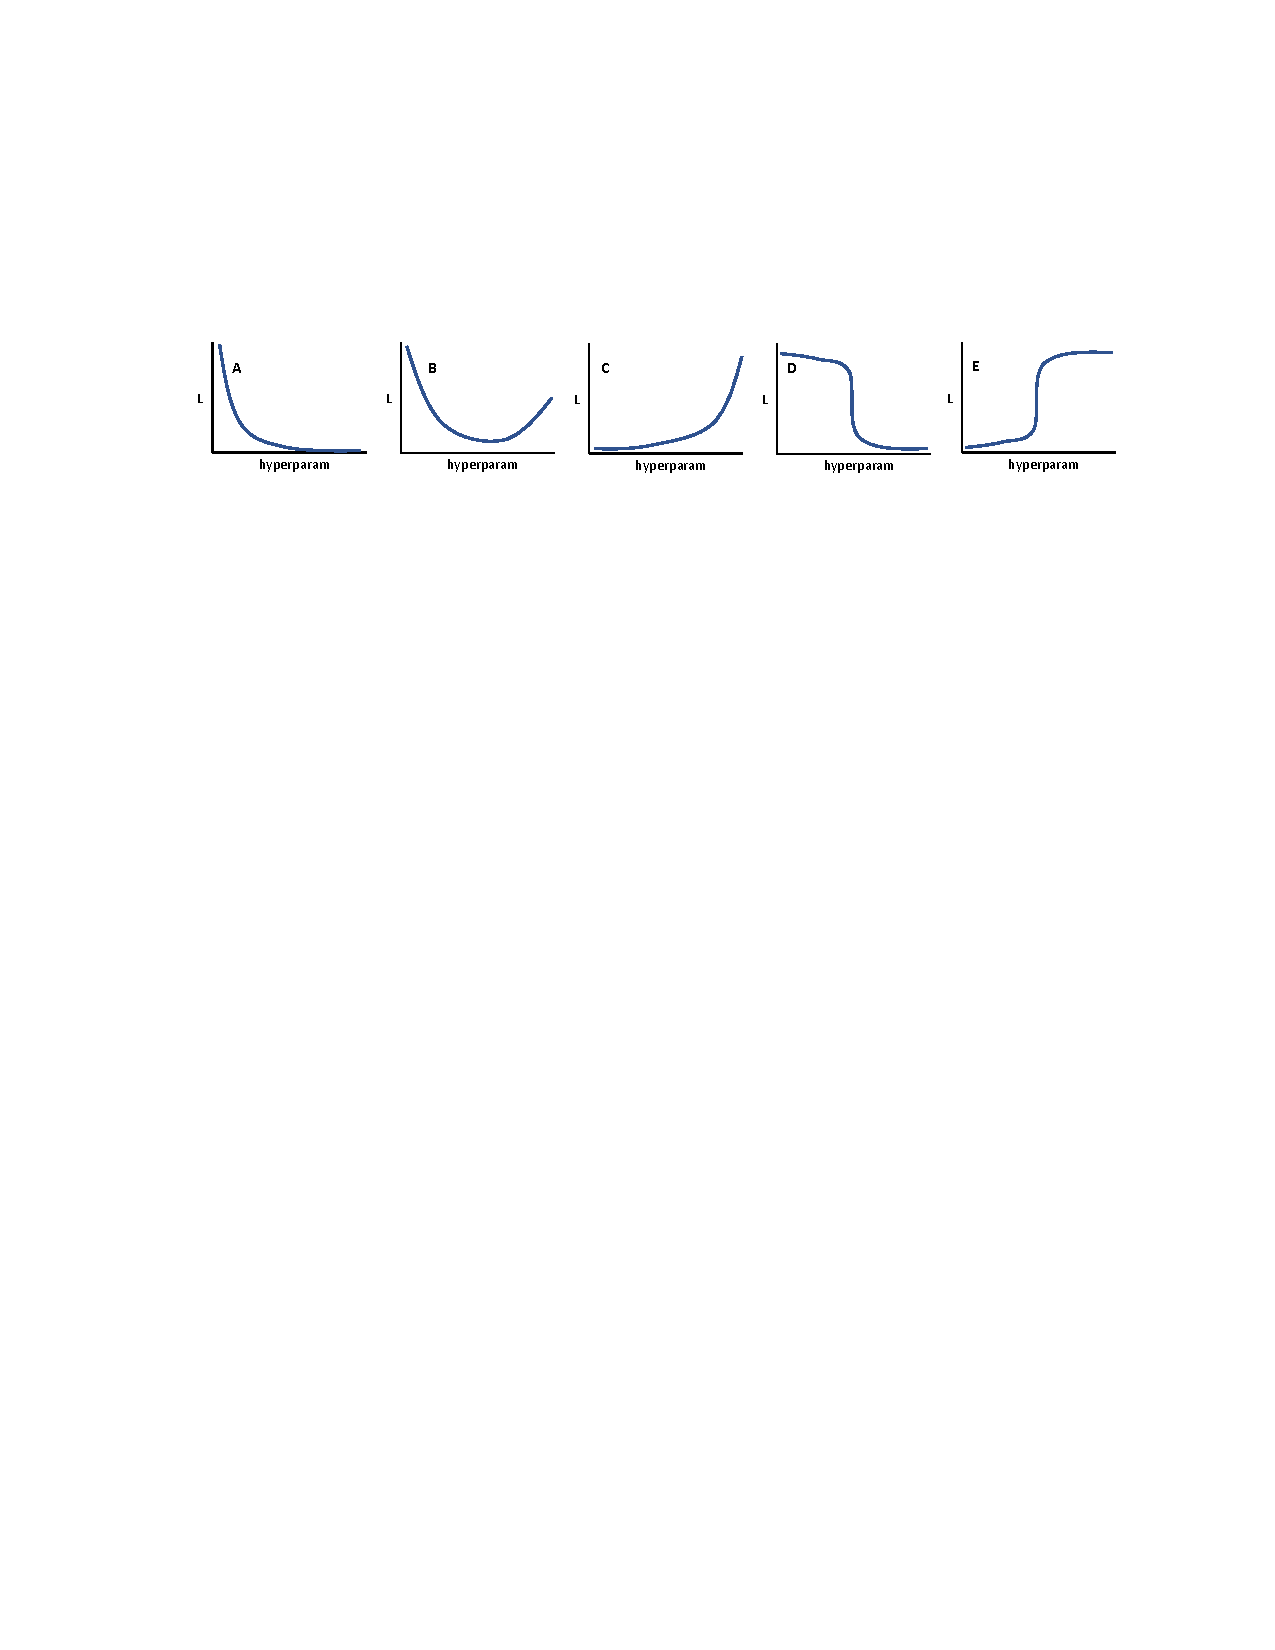
\includegraphics{images/1.pdf}
\vspace{1cm}

برای هریک از قسمت‌های زیر فقط یکی از شکل‌های A تا E را انتخاب کنید که محتمل‌ترین تغییر رفتار تابع زیان بر اساس تغییرات مقدار Hyperparameter
است. هم‌چنین، دلیل انتخاب خود را توضیح دهید.
\begin{enumerate}
    \item[(الف)] $k$: تعداد همسایگان در الگوریتم $k$ نزدیک‌ترین همسایه
    (kNN)
\begin{itemize}
        \item میزان خطا با تغییر $k$
{\latin      
\tikz\draw[thick](0,0)circle(0.15); A \quad
\tikz\draw[thick](0,0)circle(0.15); B \quad
\tikz\draw[thick](0,0)circle(0.15); C \quad
\tikz\draw[thick](0,0)circle(0.15); D \quad
\tikz\draw[thick](0,0)circle(0.15); E
}
\end{itemize}
\vspace{1.5cm}
\item[(ب)] $d$: عمق یک درخت تصمیم‌
\begin{itemize}
        \item زیان آموزش \lr{ Training Loss}
{\latin      
\tikz\draw[thick](0,0)circle(0.15); A \quad
\tikz\draw[thick](0,0)circle(0.15); B \quad
\tikz\draw[thick](0,0)circle(0.15); C \quad
\tikz\draw[thick](0,0)circle(0.15); D \quad
\tikz\draw[thick](0,0)circle(0.15); E
}
\vspace{1.5cm}
        \item زیان تست \lr{ Test Loss}
{\latin      
\tikz\draw[thick](0,0)circle(0.15); A \quad
\tikz\draw[thick](0,0)circle(0.15); B \quad
\tikz\draw[thick](0,0)circle(0.15); C \quad
\tikz\draw[thick](0,0)circle(0.15); D \quad
\tikz\draw[thick](0,0)circle(0.15); E
}
\vspace{1.5cm}
\end{itemize}
\item[(پ)] $\alpha$ نرخ یادگیری
\lr{Learning Rate}
در رگرسیون لاجستیک 
\lr{Logistic Regression}
\begin{itemize}
        \item زیان آموزش \lr{ Training Loss}
{\latin      
\tikz\draw[thick](0,0)circle(0.15); A \quad
\tikz\draw[thick](0,0)circle(0.15); B \quad
\tikz\draw[thick](0,0)circle(0.15); C \quad
\tikz\draw[thick](0,0)circle(0.15); D \quad
\tikz\draw[thick](0,0)circle(0.15); E
}
\vspace{1.5cm}
        \item زیان تست \lr{ Test Loss}
{\latin      
\tikz\draw[thick](0,0)circle(0.15); A \quad
\tikz\draw[thick](0,0)circle(0.15); B \quad
\tikz\draw[thick](0,0)circle(0.15); C \quad
\tikz\draw[thick](0,0)circle(0.15); D \quad
\tikz\draw[thick](0,0)circle(0.15); E
}
\vspace{1.5cm}
\end{itemize}

\item[(ت)] تعداد درختان در جنگل تصادفی \lr{Random Forest}
\begin{itemize}
        \item زیان آموزش \lr{ Training Loss}
{\latin      
\tikz\draw[thick](0,0)circle(0.15); A \quad
\tikz\draw[thick](0,0)circle(0.15); B \quad
\tikz\draw[thick](0,0)circle(0.15); C \quad
\tikz\draw[thick](0,0)circle(0.15); D \quad
\tikz\draw[thick](0,0)circle(0.15); E
}
\vspace{1.5cm}
        \item زیان تست \lr{ Test Loss}
{\latin      
\tikz\draw[thick](0,0)circle(0.15); A \quad
\tikz\draw[thick](0,0)circle(0.15); B \quad
\tikz\draw[thick](0,0)circle(0.15); C \quad
\tikz\draw[thick](0,0)circle(0.15); D \quad
\tikz\draw[thick](0,0)circle(0.15); E
}
\vspace{1.5cm}
\end{itemize}

\end{enumerate}
\end{enumerate}

\pagebreak
\hline
نام و نام خانوادگی: \hspace{8cm} شماره دانشجویی:
\hline
\vspace{0.5cm}
\textbf{خوشه خوشه}

در این مسئله می‌خواهیم به بررسی الگوریتم خوشه بندی
k-means بپردازیم. فرض کنید \(X = {x_1, x_2, ..., x_n}\) داده‌های ما باشد و $\gamma$ یک ماتریس Indicator باشد به این صورت که $\gamma_{ij} = 1$ اگر \(x_i\) متعلق به خوشه j ام باشد و در غیر این صورت برابر ۰ است. فرض کنید $\mu_1, ..., \mu_k$ میانگین خوشه ها باشند. اعوجاج J برای داده‌ها به صورت زیر محاسبه می‌شود :
\[J(\gamma, \mu_1, ..., \mu_k) = n\sum_{j=1}^{k}\sum_{i=1}^{n}\gamma_{ij}\lVert x_i - \mu_j \rVert^2\]
همچنین \(C = 1, ..., k\) را به عنوان مجموعه خوشه ها در نظر بگیرید.
\begin{enumerate}
\item
آیا k-means نسبت به انتخاب نقاط اولیه حساس است، یعنی پاسخ آن بر اساس مجموعه‌ی نقاط اولیه تغییر می‌کند؟ اگر بله یک مثال ارائه کنید و اگر خیر، اثبات کنید.
\vspace{4cm}
\item
نشان دهید که الگوریتم k-means در زمان متناهی قدم به پایان می‌رسد. (راهنمایی: نشان دهید $J$ تعداد محدودی حالت دارد.)
\vspace{7cm}
\item
اگر ابعاد داده نسبت به تعداد نمونه‌ها خیلی زیاد باشد و عملا نمونه‌ها در یک فضای بزرگ پراکنده باشند، برای بهبود خوشه‌بندی از چه روشی استفاده می‌کنید؟
\pagebreak
\item
نشان دهید که کمینه J یک تابع غیرافزایشی بر حسب k یا همان تعداد خوشه هاست. در این صورت آیا انتخاب مقدار هایپرپارامتر $k$ بر اساس کمینه‌کردن مقداز $J$ ایده‌ی خوبی است؟ اگرنه، چه ایده‌ی بهتری دارید؟
\vspace{7cm}
\item
فرض کنید $\hat{x}$ میانگین داده‌های نمونه باشد. مقادیر زیر را در نظر بگیرید.
\[T(X) = \frac{\sum_{i=1}^{n}\lVert x_i - \hat{x}\rVert^2}{n}\]
\[W_j(X) = \frac{\sum_{i=1}^{n}\gamma_{ij}\lVert x_i - \mu_j\rVert^2}{\sum_{i=1}^{n}\gamma_{ij}}\]
\[B(X) = \sum_{j=1}^{k}\frac{\sum_{i=1}^{n}\gamma_{ij}}{n}\r\lVert \mu_j - \hat{x} \rVert^2\]
در اینجا \(T(X)\) نشان دهنده انحراف کلی، \(W_j(X)\) انحراف 
درون خوشه‌ای و \(B(X)\) انحراف بین خوشه‌ای است.
رابطه‌ی بین این ۳ مقدار به چه صورت است؟
نشان دهید که k-means میتواند به عنوان کمینه کننده میانگین وزن دار مقادیر درون خوشه‌ای و به طور تقریبی بیشینه کردن انحراف بین خوشه‌ای دیده شود.
\vspace{7cm}
\end{enumerate}
\pagebreak
\hline
نام و نام خانوادگی: \hspace{8cm} شماره دانشجویی:
\hline
\vspace{0.5cm}
\textbf{خلاف شیب}

در بسیاری از سناریوهای دنیای واقعی، داده‌های ما دارای میلیون‌ها بُعد هستند، اما یک نمونه خاص فقط دارای صدها ویژگی غیرصفر است. به عنوان مثال، در تحلیل اسناد با تعداد کلمات به عنوان ویژگی‌ها، ممکن است فرهنگ لغت ما میلیون‌ها کلمه داشته باشد، اما یک سند خاص فقط دارای صدها کلمه منحصر به فرد است. در این سؤال، می‌خواهیم نرم \lr{\(\ell_2\)-Regularized Stochastic Gradient Descent (SGD)} برای زمانی که داده‌های ورودی ما sparse است را کارا کنیم. به خاطر داشته باشید که در Regression Logistic \(\ell_2\) ، می‌خواهیم تابع هدف زیر را کمینه کنیم (در این مسئله برای سادگی \(w_0\) حذف شده است):

\begin{latin}
\[
F(\mathbf{w}) = \frac{1}{N} \sum_{j=1}^N l(\mathbf{x}^{(j)}, y^{(j)}, \mathbf{w}) + \frac{\lambda}{2} \sum_{i=1}^d w_i^2
\]
\end{latin}

که در آن \(l(\mathbf{x}^{(j)}, y^{(j)}, \mathbf{w})\) تابع هدف است:

\begin{latin}
    
\[
l(\mathbf{x}^{(j)}, y^{(j)}, \mathbf{w}) =\ln \left( 1 + \exp \left( \sum_{i=1}^d w_i x_i^{(j)} \right)\right) - y^{(j)} \left( \sum_{i=1}^d w_i x_i^{(j)} \right) 
\]
\end{latin}

و باقی مانده‌ی جمع، میزان Penalty Regularization خواهد بود.

وقتی روی نقطه \((\mathbf{x}^{(j)}, y^{(j)})\) \lr{SGD} انجام می‌دهیم، تابع هدف را به صورت زیر تقریب می‌زنیم:

\begin{latin}
    
\[
F(\mathbf{w}) \approx l(\mathbf{x}^{(j)}, y^{(j)}, \mathbf{w}) + \frac{\lambda}{2} \sum_{i=1}^d w_i^2
\]
\end{latin}

% \textbf{تریف :sparse} فرض کنید داده‌های ورودی ما دارای \(d\) ویژگی هستند، به عبارت دیگر \(\mathbf{x}^{(j)} \in \mathbb{R}^d\). در این مسئله، سناریویی را در نظر خواهیم گرفت که \(\mathbf{x}^{(j)}\) تنک باشد. به عبارت دیگر، فرض کنید \(s\) میانگین تعداد عناصر غیرصفر در هر نمونه باشد. ما زمانی که \(s \ll d\) باشد، می‌گوییم داده‌ها sparse هستند. در سوالات بعدی، \textbf{پاسخ شما باید در صورت امکان sparse \(\mathbf{x}^{(j)}\) را در نظر بگیرد}. (نکته: هنگامی که از ساختار داده sparse استفاده می‌کنیم، می‌توانیم در زمان \(O(s)\) عناصر غیرصفر را بررسی کنیم، در حالی که یک ساختار داده متراکم به زمان \(O(d)\) نیاز دارد.)

\begin{enumerate}
    \item 

 ابتدا حالت \(\lambda = 0\) را در نظر بگیرید. قانون به‌روزرسانی SGD برای \(w_i\) را هنگامی که \(\lambda = 0\) است، با استفاده از اندازه گام \(\eta\) و با توجه به نمونه \((\mathbf{x}^{(j)}, y^{(j)})\) بنویسید.

\vspace{5cm}

\item
اگر از یک ساختار داده متراکم استفاده کنیم، میانگین پیچیدگی زمانی برای به‌روزرسانی \(w_i\) هنگامی که \(\lambda = 0\) است، چقدر است؟ اگر از یک ساختار داده تنک استفاده کنیم، چطور؟ پاسخ خود را در یک یا دو جمله توضیح دهید.

\vspace{5cm}

\item
 اکنون حالت کلی را که \(\lambda > 0\) در نظر بگیرید. قانون به‌روزرسانی SGD برای \(w_i\) را هنگامی که \(\lambda > 0\) است، با استفاده از اندازه گام \(\eta\) و با توجه به نمونه \((\mathbf{x}^{(j)}, y^{(j)})\) بنویسید.

\vspace{5cm}

\item
  اگر از یک ساختار داده متراکم استفاده کنیم، میانگین پیچیدگی زمانی برای به‌روزرسانی \(w_i\) هنگامی که \(\lambda > 0\) است، چقدر است؟

\vspace{5cm}

\item
 فرض کنید \(\mathbf{w}^{(t)}_i\) بردار وزن بعد از به‌روزرسانی \(t\)ام باشد. اکنون فرض کنید که \(k\) به‌روزرسانی SGD روی \(\mathbf{w}\) با استفاده از نمونه‌های \((\mathbf{x}^{(t+1)}, y^{(t+1)}), \cdots , (\mathbf{x}^{(t+k)}, y^{(t+k)})\) انجام می‌دهیم، که در آن \(x_i^{(j)} = 0\) برای هر نمونه در دنباله باشد (یعنی ویژگی \(i\)ام برای تمام نمونه‌ها در دنباله صفر است). وزن جدید \(\mathbf{w}^{(t+k)}_i\) را بر حسب \(\mathbf{w}^{(t)}_i\)، \(k\)، \(\eta\)، و \(\lambda\) حساب کنید.

\vspace{5cm}

\item
با استفاده از پاسخ خود در قسمت قبل، یک الگوریتم کارا برای \lr{Regularized SGD} ارائه دهید زمانی که از ساختار داده sparse استفاده می‌کنیم. میانگین پیچیدگی زمانی به‌ازای هر نمونه چقدر است؟\\ \textbf{راهنمایی:} چه زمانی نیاز به به‌روزرسانی \(w_i\) دارید؟
\end{enumerate}

\pagebreak
\hline
نام و نام خانوادگی: \hspace{8cm} شماره دانشجویی:
\hline
\vspace{0.5cm}
\textbf{خرد جمعی}

می‌دانیم که Adaboost یک دسته‌بند \(H\) را با استفاده از جمع وزن‌دار یادگیرنده‌های ضعیف \(h_t\) به صورت زیر یاد می‌گیرد:

\begin{latin}
    
\[
H(x) = \operatorname{sgn} \left( \sum_{t=1}^T \alpha_t h_t(x) \right)
\]
\end{latin}


در این سوال، ما از درخت‌های تصمیم به عنوان یادگیرنده‌های ضعیف خود استفاده می‌کنیم، که یک نقطه را به عنوان \(\{1, -1\}\) بر اساس دنباله‌ای از \lr{threshold}ها روی ویژگی‌های آن (اینجا \(x, y\)) طبقه‌بندی می‌کنند.

در سوالات زیر فرض کنید 
 که در صورت برابری امتیاز برای کلاس مثبت و منفی، خروجی دسته‌بندها به طور دلخواه تعیین می‌شود.
\vspace{-5mm}
\begin{enumerate}
\item
فرض کنید یادگیرنده‌های ضعیف ما درخت‌های تصمیم با عمق 1 هستند (\lr{Decision Stumps})، که خطای آموزشی وزن‌دار را کمینه می‌کنند. با استفاده از مجموعه داده زیر، مرز تصمیمی که توسط \(h_1\) یاد گرفته شده است را ترسیم کنید.
\vspace{-5mm}
\begin{figure}[H]
    \latin
    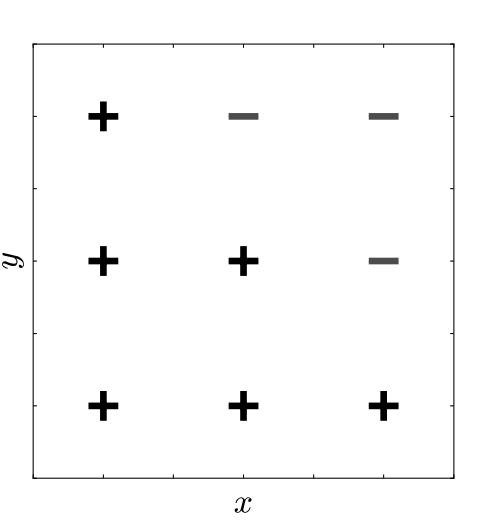
\includegraphics[width=0.28\linewidth,left]{images/2-1.png}
\end{figure}
\vspace{-5mm}
\item
 در مجموعه داده‌ی زیر، نقطه(های) با بیشترین وزن در \lr{iteration} دوم را مشخص و مرز تصمیمی که توسط \(h_2\) یاد گرفته شده است را ترسیم کنید.
 \vspace{-5mm}
\begin{figure}[H]
    \latin
    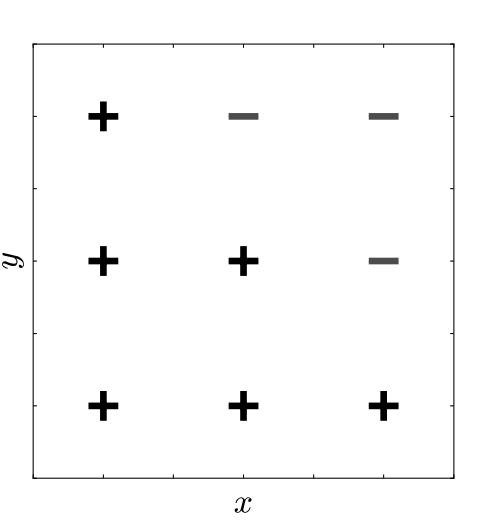
\includegraphics[width=0.28\linewidth,left]{images/2-1.png}
\end{figure}
\vspace{-5mm}
\item
در مجموعه داده‌ی زیر، مرز تصمیم \(H = \operatorname{sgn} (\alpha_1 h_1 + \alpha_2 h_2)\) را ترسیم کنید. (راهنمایی: نیازی به محاسبه صریح \(\alpha\) ها نیست).
\vspace{-5mm}
\begin{figure}[H]
    \latin
    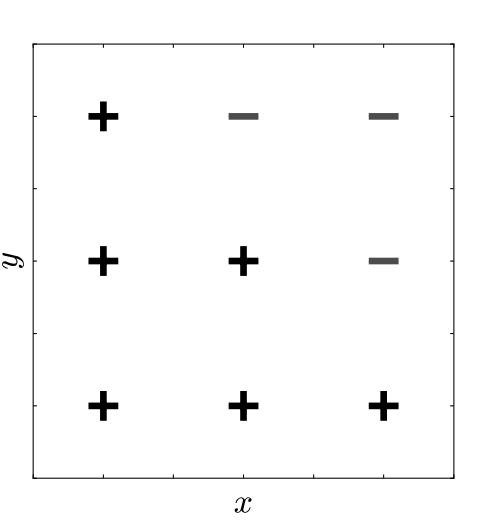
\includegraphics[width=0.28\linewidth,left]{images/2-1.png}
\end{figure}
\vspace{-5mm}
\item
اکنون فرض کنید که یادگیرنده‌های ضعیف ما درخت‌های تصمیم با عمق حداکثر 2 هستند، که خطای آموزشی وزن‌دار را کمینه می‌کنند. با استفاده از مجموعه داده‌ی زیر، مرز تصمیمی که توسط \(h_1\) یاد گرفته شده است را ترسیم کنید.
\begin{figure}[H]
    \latin
    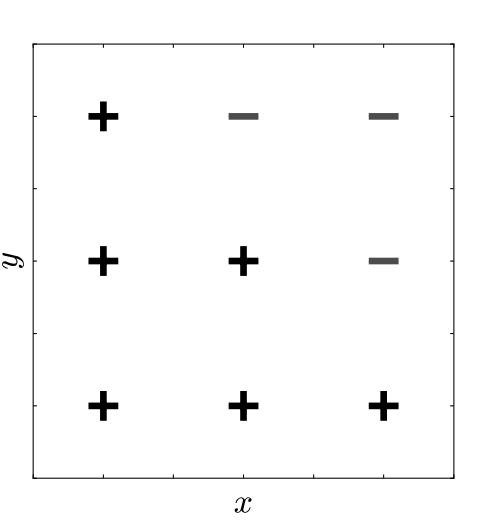
\includegraphics[width=0.28\linewidth,left]{images/2-1.png}
\end{figure}
\vspace{-5mm}
\item
 در مجموعه داده‌ی زیر، نقطه(ها) با بیشترین وزن در \lr{iteration} دوم را دایره بکشید و مرز تصمیمی که توسط \(h_2\) یاد گرفته شده است را ترسیم کنید.
\vspace{-5mm}
\begin{figure}[H]
    \latin
    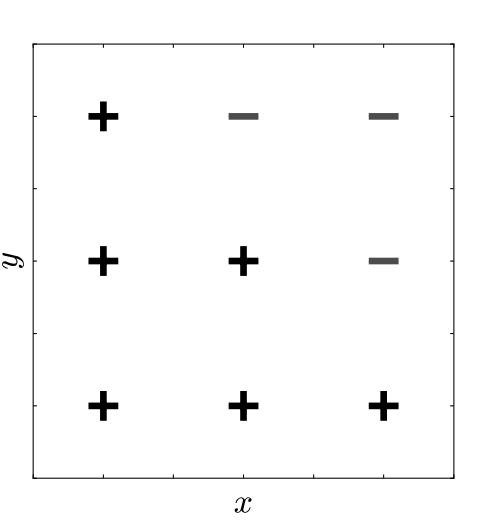
\includegraphics[width=0.28\linewidth,left]{images/2-1.png}
\end{figure}
\vspace{-5mm}
\item
در مجموعه داده‌ی زیر، مرز تصمیم \(H = \operatorname{sgn} (\alpha_1 h_1 + \alpha_2 h_2)\) را ترسیم کنید. (راهنمایی: نیازی به محاسبه صریح \(\alpha\) ها نیست).
\vspace{-5mm}
\begin{figure}[H]
    \latin
    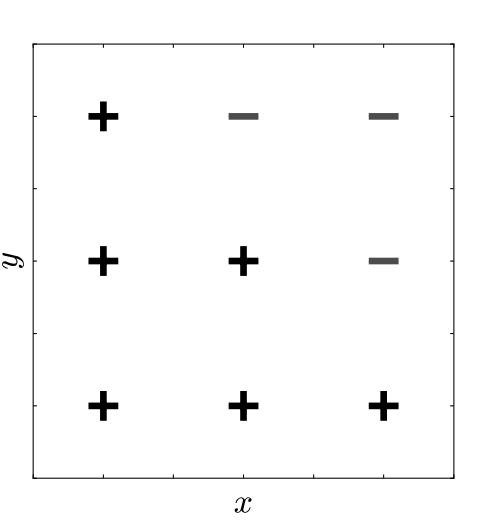
\includegraphics[width=0.28\linewidth,left]{images/2-1.png}
\end{figure}
\end{enumerate}
\pagebreak
\hline
نام و نام خانوادگی: \hspace{8cm} شماره دانشجویی:
\hline
\vspace{0.5cm}
\textbf{Tikhonov}

تابع هزینه مسئله رگرسیون خطی به صورت زیر تعریف می‌شود:
\[\mathbb{L}_1(w) = \lVert y - Xw \rVert_2^2\]
همانطور که در درس دیدید، می‌توانیم چند عنصر دیگر به عنوان Term Regularization به این تابع هزینه اضاقه کنیم. در این صورت خواهیم داشت:
\[\mathbb{L}_2(w) = \lVert y - Xw \rVert_2^2 + \lVert \Gamma w \rVert_2^2\]
که به \(\Gamma\)، matrix Tikhonov می‌گویند. این حالت کلی مسئله regression ridge است که در اینجا به جای \(\lambda\), از یک ماتریس استفاده می‌کنیم. 
برای آموزش مدل رگرسیون خطی خود، می‌خواهیم از تکنیکی به نام \(drop out\) استفاده کنیم. این تکنیک برای ورودی \(d\) بعدی، هر ویژگی را با احتمال \(p\) نگه داشته و در غیر این صورت برابر صفر خواهد شد. با استفاده از این تکنیک، تابع هزینه به شکل زیر تغییر خواهد کرد :
\[\mathbb{L}_3(w) = \mathbb{E}_{D\textasciitilde Bernouli(p)}[\lVert y - (D \odot X)\hat{w} \rVert_2^2]]\]
توجه کنید در اینجا \(\hat{w}\) پارامتر های پیدا شده توسط مدلی است که با \(dropout\) آموزش داده شده است. همچنین ضرب \(\odot\)، ضرب wise element می‌باشد.
\begin{enumerate}
    \item ابتدا معادله نرمال برای حل مساله‌ی minimization بدون توجه به \(dropout\) به دست آورید. در اینجا شما مانند دیگر مسئله های رگرسیون، باید وزن های بهینه را با استفاده از مشتق و ... با استفاده از تابع هزینه به دست آورید.
    \vspace{6cm}
    \item یک شرط ساده، کافی و لازم برای ماتریس \(\Gamma\) بیان کنید که تضمین کند تابع هزینه یک جواب منحصر به فرد و بهینه برای \(\hat{w}\) دارد.
    \vspace{9cm}

    \item حال اثبات کنید هنگام استفاده از تکنیک \(dropout\),  می‌توان تابع هزینه را به شکل زیر بازنویسی کرد :
    \[\mathbb{L}(w) = \lVert y - pX\hat{w} \rVert_2^2 + p(1 - p)\lVert \hat{\Gamma}\hat{w} \rVert_2^2\]
    به طوری که \(\hat{\Gamma}\) یک ماتریس قطری بوده که عنصر \(j\) ام قطری این ماتریس، برابر نرم ستون \(j\) ام ماتریس دادگان \(X\) می باشد.
        \vspace{9cm}

    \item فرض کنید \(\Gamma\) معکوس پذیر باشد. با یک تغییر متغیر سعی کنید تا تابع هزینه گفته شده در حالت بدون \(dropout\)را به صورت تابع هزینه مسئله regression ridge بازنویسی کنید :
    \[\mathbb{L}(\hat{w}) = \lVert y - \hat{X}\hat{w} \rVert_2^2 + \lambda \lVert \hat{w} \rVert_2^2\]
\end{enumerate}
\pagebreak
\hline
نام و نام خانوادگی: \hspace{8cm} شماره دانشجویی:
\hline
\vspace{0.5cm}
\textbf{اصلی}

در یک شرکت بزرگ کاریابی کار می‌کنید. هر فرد یک پروفایل دارد که بعضی ویژگی‌های آن (نظیر سن، آخرین حقوق) عدد پیوسته و بعضی ویژگی‌های دیگر (نظیر رشته‌ی تحصیلی) Categorical است. 
همچنین بعضی از ویژگی‌ها (نظیر آشنایی با هریک از زبان‌های برنامه‌نویسی) به صورت صفر و یک درج شده است. 

\begin{enumerate}
\item می‌خواهید برای هر کاربر جدید که پروفایل خود را تکمیل کرده‌است، یک مبلغ حقوق تخمین بزنید. از چه الگوریتمی استفاده می‌کنید؟ چه تغییری روی ویژگی‌ها می‌دهید؟ برای هریک از ویژگی‌ها از چه پیش‌پردازشی استفاده می‌کنید؟ جزئیات را توضیح دهید.
\vspace{5cm}
\item
حال می‌خواهید داده‌های این شرکت را به صورت یک نمودار نمایش دهید. برای این کار تصمیم دارید از تحلیل مولفه‌های اصلی (PCA) استفاده کنید.
آیا به نظر شما تغییر مقیاس ویژگی‌ها لازم است؟ اگر بله، چرا؟ و چطور این کار را انجام می‌دهید؟ اگر خیر، دلیل‌ شما چیست؟
\vspace{5cm}
\item
فرض کنید ماتریس کوواریانس زیر را داشته باشید. چطور از روی آن مولفه‌های اصلی را مشخص می‌کنید؟ محاسبات خود را بنویسید.
{\latin
\centering
$C=$\begin{bmatrix}
3 & -4\\
-4 & 3
\end{bmatrix}
}
\vspace{5cm}
\item
فرض کنید می‌خواهید با PCA ابعاد داده‌هاهای شرکت را با بردن آن‌ها فضای جدیدی کاهش دهید که عمده‌ی اطلاعات حفظ شود. چطور تعداد بعدهای فضای جدید را مشخص می‌کنید؟
\vspace{6cm}
\item
ثابت کنید تصویرکردن داده‌ها توسط بردارویژه‌‌ی با بزرگ‌ترین مقدار ویژه‌ی ماتریس کوواریانس، واریانس داده‌های تصویرشده را بیشینه می‌کند.
\vspace{6cm}
\item
به دل‌خواه یک مساله‌ی زیبای یادگیری ماشین بنویسید و آن را حل کنید. نمره‌ی این بخش به زیبایی و منحصر به فرد بودن مساله‌ و درستی راه‌حل شما اختصاص می‌یابد.

\end{enumerate}

\end{document}
